\documentclass[10pt,a4paper]{amsart}
\usepackage{amsmath,amssymb,amsthm,graphicx}
\usepackage{amsmath}
\usepackage{amsfonts}
\usepackage{amssymb}
\usepackage{graphicx}
\usepackage{float}
\usepackage{caption}
\usepackage{pgf,tikz}
\usetikzlibrary{arrows}
\usepackage{verbatim}
\usepackage{hyperref}

\definecolor{ffttww}{rgb}{1,0.2,0.4}
\definecolor{uuuuuu}{rgb}{0.27,0.27,0.27}
\definecolor{cqcqcq}{rgb}{0.75,0.75,0.75}
\definecolor{wwqqcc}{rgb}{0.4,0,0.8}

\newcommand{\R}{\mathbb{R}}
\newcommand{\N}{\mathbb{N}}
\newcommand{\HH}{\mathcal{H}}
\newcommand{\RR}{\mathcal{R}}
\newcommand{\A}{\mathcal{A}}
\newcommand{\B}{\mathcal{B}}
\newcommand{\est}{\emptyset}
\newtheorem{theorem}{Theorem}
\newtheorem{proposition}{Proposition}
\newtheorem{corollary}{Corollary}
\newtheorem{lemma}{Lemma}
\newtheorem{definition}{Definition}
\newtheorem{jel}{Notation}
\newtheorem{conj}{Conjecture}
\title{Uniform axis-parallel strip hypergraphs with no2-shallow hitting set}
\author{Balázs Bursics, Bence Csonka, Luca Szepessy}
\date{arxiv:2307.12154v3; CC BY 4.0}
\begin{document}
\maketitle
\noindent\textit{Editorial note.} The original two PNG figures are included with their basenames. Their black lines are visible on the white PDF page; the transparent images were also checked in the official PDF page13 for the local cluster sizes.\par\medskip
\noindent\textit{Editorial note.} Source542 puts conv around projected point sets inside a cardinality equal to a. The surrounding sentence535 and the original figure clearly specify a of the2a individual X\_i,1 points on each side of the anchor; cardinality of a real interval is not intended. Original wording is retained with this clarification.\par\medskip
\noindent\textit{Editorial note.} The construction may choose distinct x- and y-coordinates within every cluster. This preserves all strict cluster-order inequalities and lets a strip with fewer than m captured points be enlarged to exactly m, one point at a time. This is the extension step already invoked at592 and needed at545.\par\medskip
\noindent\textit{Editorial note.} The source figures give |X|=2a, |B|=|C|=m-2a, |D|=2a-1, |E|=|F|=m-2a-b+1=a-b/2, |G|=|H|=b, |I|=m-2b, and |J|=|K|=2b. These are transcribed here for legibility; the original figures and prose remain the author proof.\par\medskip
\noindent\textit{Editorial note.} The auxiliary clusters for distinct local gadgets occupy separate horizontal bands outside all global J\_i strips, and the complete local gadget stays inside its own reserved vertical I interval, as required by source539/547.\par\medskip
\noindent\textit{Editorial scope.} One geometric nonexistence construction for2-shallow hitting sets in m-uniform axis-parallel-strip hypergraphs for sufficiently large m. The complete local and global construction is counted, including both source figures. No3-shallow upper bound, polychromatic theorem or arithmetic-progression result is counted.\par\medskip
\noindent\textit{Allowed standard prerequisites (editorial).}\begin{itemize}
\item Finite planar range hypergraphs and general position. An axis-parallel strip captures exactly the input points between two vertical or two horizontal lines. The finitely many freely placed points can have distinct x- and y-coordinates while satisfying the author strict inequalities.. Choose strip boundaries between coordinates, and enlarge a captured set of at most m points to exactly m points by moving a boundary when needed.
\item Elementary finite counting and set intersections. Track the exact cluster sizes and the consequences of every captured m-edge having one or two selected vertices.
\end{itemize}\medskip
\begin{definition} Denote by $H_{\ge m}$ or simply $H_m$ the hypergraph obtained from $H$ by deleting all hyperedges of size smaller than $m$, and denote by $H_{=m}$ the hypergraph consisting of the hyperedges of $H$ with size exactly $m$. Similarly, for a hypergraph family $\mathcal{H}$ let $\HH_m=\HH_{\ge m}=\{H_{\ge m}:H\in\HH\}$ and $\HH_{=m}=\{H_{=m}:H\in\HH\}$.
\end{definition}

\begin{definition}
 Let $H=(V,E)$ be a hypergraph, a $U\subset V$ vertex set $U\subset V$ is a {\it c-shallow hitting set} for a positive integer $c$ if for every hyperedge $e\in E$: $1\le|e\cap U|\le c.$
\end{definition} 

\begin{definition} Denote by $\A$ the hypergraph family which consists of those hypergraphs $H=(V,E)$ for which $V\subset \R^2$ is finite, and the edges are induced by axis-parallel strips: every $e\in E$ edge can be presented in the form $V\cap\{(x,y)\in\R^2: x_0<x<x_1\}$ or $V\cap\{(x,y)\in\R^2: y_0<y<y_1\}$ for some $x_0, x_1, y_0, y_1 \in\R$. Denote by $\A^*$ its dual: the family of such hypergraphs that the vertices are axis-parallel strips, and the edges are sets consisting of the strips containing a given point $(x,y)$. 
\end{definition}

\begin{theorem}\label{strip}
For sufficiently large $m$ there is an element in $\A_{=m}$ with no 2-shallow hitting set.
\end{theorem}

\begin{proof}[Proof of Theorem~\ref{strip}]

We construct a hypergraph in $\A$ with no 2-shallow hitting sets. The main arrangement of some vertices can be seen on Figure \ref{abra1}.
\begin{figure} [h!]
    \centering
    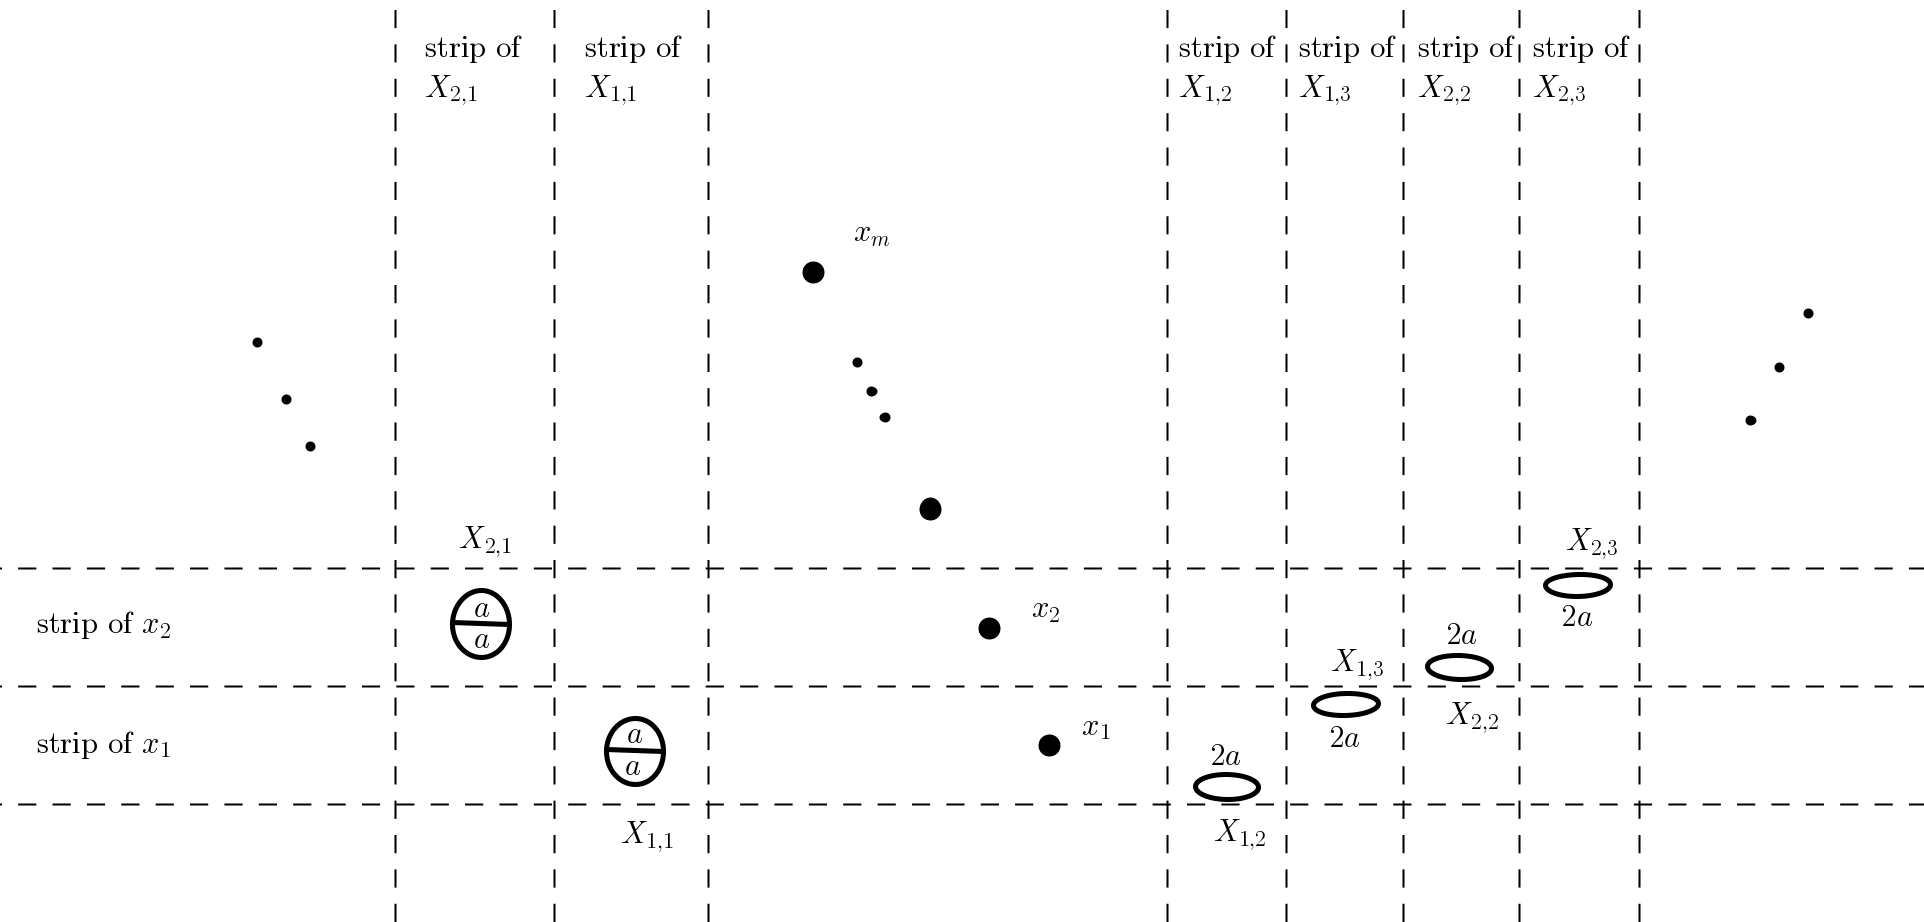
\includegraphics{abra1_en.png}
    \caption{The construction for Theorem~\ref{strip}.}
\label{abra1}
\end{figure}

\begin{comment}
\begin{figure} [h!]
    \centering
    \begin{tikzpicture}[line cap=round,line join=round,>=triangle 45,x=1.2cm,y=1.2cm]
\clip(-5.27,-1.71) rectangle (6.85,4.79);
\draw [line width=0.4pt,dash pattern=on 4pt off 4pt,domain=-5.27:6.85] plot(\x,{(--3.51-0*\x)/7.02});
\draw [line width=0.4pt,dash pattern=on 4pt off 4pt,domain=-5.27:6.85] plot(\x,{(-6-0*\x)/12});
\draw [line width=0.4pt,dash pattern=on 4pt off 4pt,domain=-5.27:6.85] plot(\x,{(--19.47-0*\x)/12.98});
\draw [line width=0.4pt,dash pattern=on 4pt off 4pt] (3,-2.21) -- (3,5.79);
\draw [line width=0.4pt,dash pattern=on 4pt off 4pt] (5.07,-2.21) -- (5.07,5.79);
\draw [line width=0.4pt,dash pattern=on 4pt off 4pt] (3.95,-2.21) -- (3.95,5.79);
\draw [line width=0.4pt,dash pattern=on 4pt off 4pt] (-1,-2.21) -- (-1,5.79);
\draw [line width=0.4pt,dash pattern=on 4pt off 4pt] (-2,-2.21) -- (-2,5.79);
\draw [line width=0.4pt,dash pattern=on 4pt off 4pt] (4.21,-2.21) -- (4.21,5.79);
\draw [rotate around={1.1:(4.63,0.35)},line width=1pt] (4.63,0.35) ellipse (0.28cm and 0.09cm);
\draw [rotate around={-1.15:(3.51,-0.35)},line width=1pt] (3.51,-0.35) ellipse (0.27cm and 0.1cm);
\draw [rotate around={90:(-1.51,-0.05)},line width=1pt] (-1.51,-0.05) ellipse (0.28cm and 0.24cm);
\draw (3.33,0.04) node[anchor=north west] [scale=0.7]{$2a$};
\draw (4.43,0.27) node[anchor=north west] [scale=0.7]{$2a$};
\draw (-5.2,0.23) node[anchor=north west] [scale=0.8]{$\text{strip of  } A$};
\draw (-5.2,1.23) node[anchor=north west] [scale=0.8]{$\text{strip of  } B$};
\draw [line width=1pt] (-1.712,-0.03)-- (-1.305,-0.04);
\draw (-1.66,0.2) node[anchor=north west] [scale=0.7]{$a$};
\draw (-1.66,-0.02) node[anchor=north west] [scale=0.7]{$a$};
\begin{scriptsize}
\fill [color=black] (2,0) circle (2.5pt);
\draw[color=black] (2.14,0.25) node {$A$};
\fill [color=black] (1.5,1) circle (2.5pt);
\draw[color=black] (1.63,1.23) node {$B$};
\fill [color=black] (1,2) circle (2.5pt);
\fill [color=black] (0.5,3) circle (2.5pt);
\fill [color=black] (0,4) circle (2.5pt);
\end{scriptsize}
\end{tikzpicture}
    \caption{The construction for Theorem~\ref{strip}.}
    \label{abra1}
\end{figure}
\end{comment}

Let $m$ be large enough, let $a= \lceil \frac{m}{3} \rceil-1$, and $b$ be 8 for $m \equiv 0 \mod 3$, 4 for $m \equiv 1 \mod 3$, and 6 for $m \equiv 2 \mod 3$, this satisfies $m=3a+ \frac{b}{2}-1$. Later we will need that $m\ge 5b$.

First we take $X_0=\{x_1,\ldots,x_m\},$ a set of $m$ points on a southeast to northwest diagonal, as in the middle of Figure \ref{abra1}. We will leave empty a vertical strip containing them. Then we assign disjoint horizontal strips containing each $x_i$, and in all of these horizontal strips, we take 3 sets of points $X_{i,1},X_{i,2},X_{i,3}$ of size $2a$ as shown on Figure \ref{abra1}, reserving disjoint vertical strips containing each of these sets, and with all points from $X_{i,2}$ and $a$ points from $X_{i,1}$ having smaller $y$-coordinates than $x_i$, and all points from $X_{i,3}$ and the other $a$ points from $X_{i,1}$ having larger $y$-coordinates than $x_i$. 

More precisely, the following properties are needed:

Take $3m+1$ pairwise disjoint closed intervals $I_1,I_2,\ldots,I_{3m+1}$ on the $x$-axis, these correspond to the strips of $X_0$ and $\{X_{i,j}\}_{1\le i\le m, 1\le j\le3}$. Take $m$ pairwise disjoint intervals on the $y$-axis, $J_1,\ldots,J_m$, these correspond to the strips of $x_1,\ldots,x_m$. Let $X_0$ be a set of $m$ points such that $\mathrm{conv}(\mathrm{proj}_1(X_0))\subseteq I_{3m+1}$ and $\mathrm{proj}_2(x_i)\in\mathrm{int(J_i)} \, (1\le i\le m).$ Let $\{X_{i,j}\}_{1\le i\le m, 1\le j\le3}$ be sets of $2a$ points each such that $\mathrm{conv}(\mathrm{proj}_1(X_{i,j}))\subseteq I_{(i-1)\cdot3+j}$ and \\
$\text{conv}(\text{proj}_2(X_{i,j}))\subseteq J_i\cap (\text{proj}_2(x_i),\infty)\hfill\text{ if } j=3,$\\
$\text{conv}(\text{proj}_2(X_{i,j}))\subseteq J_i\cap (-\infty,\text{proj}_2(x_i))\hfill\text{ if } j=2,$\\
$|\text{conv}(\text{proj}_2(X_{i,j}))\cap J_i\cap (\text{proj}_2(x_i),\infty)|=|\text{conv}(\text{proj}_2(X_{i,j}))\cap J_i\cap (-\infty,\text{proj}_2(x_i))|=a\text{ if } j=1.$


It is enough to show that we can place additional points in the vertical strips in such a way that it forces the original set of $2a$ points to contain a point from a 2-shallow hitting set. Indeed, if this is the case, there is an element in $X_0$ from the hitting set, say $x_i,$ and $X_{i,1},X_{i,2},$ and $X_{i,3}$ each contain a point from the hitting set. Then there is a horizontal strip with $3a+1\le m$ vertices which contains at least 3 points from the hitting set, namely, $\R\times[\text{proj}_2(x_i),\max(J_i)]$ or $\R\times[\min(J_i),\text{proj}_2(x_i)]$, depending on which half of $X_{i,1}$ contains a point from the hitting set, a contradiction.

For each $X\in\{X_{i,j}: 1\le i\le m, \,1\le j\le3\}$, the construction of this arrangement in a vertical strip is shown on Figure \ref{gigasok}. These points are once again placed in separate horizontal strips for each $X_{i,j}$ (that is, the convex hulls of their projection to the $y$ axis are pairwise disjoint closed intervals, disjoint even with $J_1,\ldots,J_m$). Fix $X\in\{X_{i,j}: 1\le i\le m, \,1\le j\le3\},$ we show that the needed arrangement indeed exists. Take 10 sets of points, $B,C,D,\ldots,K,$ with cardinalities shown on Figure \ref{gigasok}, so that for any elements $(x^B,y^B)\in B, (x^C,y^C)\in C, \ldots, (x^K,y^K)\in K$ and $(x^X,y^X)\in X$ we have 

\begin{center}
    $x^I<x^K<x^J<x^G<x^E<x^D<x^H<x^F<x^C<x^X<x^B,$

    $y^X<y^K<y^J<y^I<y^G<y^H<y^E<y^B<y^D<y^C,$

    $y^H<y^F<y^B.$
\end{center}

\noindent Therefore, if we take neighboring strips on Figure \ref{gigasok}, then the union of the contained sets is captured by an axis-parallel strip.  

Moreover, we arrange the points of $B=\{b_1,b_2,\ldots,b_{m-2a}\}$ and $C=\{c_1,c_2,\ldots,c_{m-2a}\}$ on a diagonal line such that for $b_k=(x_k^B,y_k^B)$ and $c_l=(x_l^C,y_l^C)$ $(1\le k,l \le m-2a)$ we have

\begin{center}
    $x_{m-2a}^C<x_{m-2a-1}^C<\ldots<x_1^C<x_{m-2a}^B<x_{m-2a-1}^B<\ldots<x_1^B,$

    $y_1^B<y_2^B<\ldots<y_{m-2a}^B<y_1^C<y_2^C<\ldots<y_{m-2a}^C.$
\end{center}

\noindent This implies that if we take $B'=\{b_k, b_{k+1},\ldots,b_{m-2a}\}$, the last few elements of $B$, and $C'=\{c_1,c_2,\ldots,c_l\}$, the first few elements of $C,$ then both $B'\cup C'\cup D$ and $B'\cup C'\cup X$ are captured by an axis-parallel strip.

%\begin{figure} [h!]
%    \centering
%    \includegraphics{abrasok.png}
%    \caption{Egy $2a$ pontból álló kupac sávja}
    %\label{fig:my_label}
%\end{figure}

\begin{figure} [h!]
    \centering
    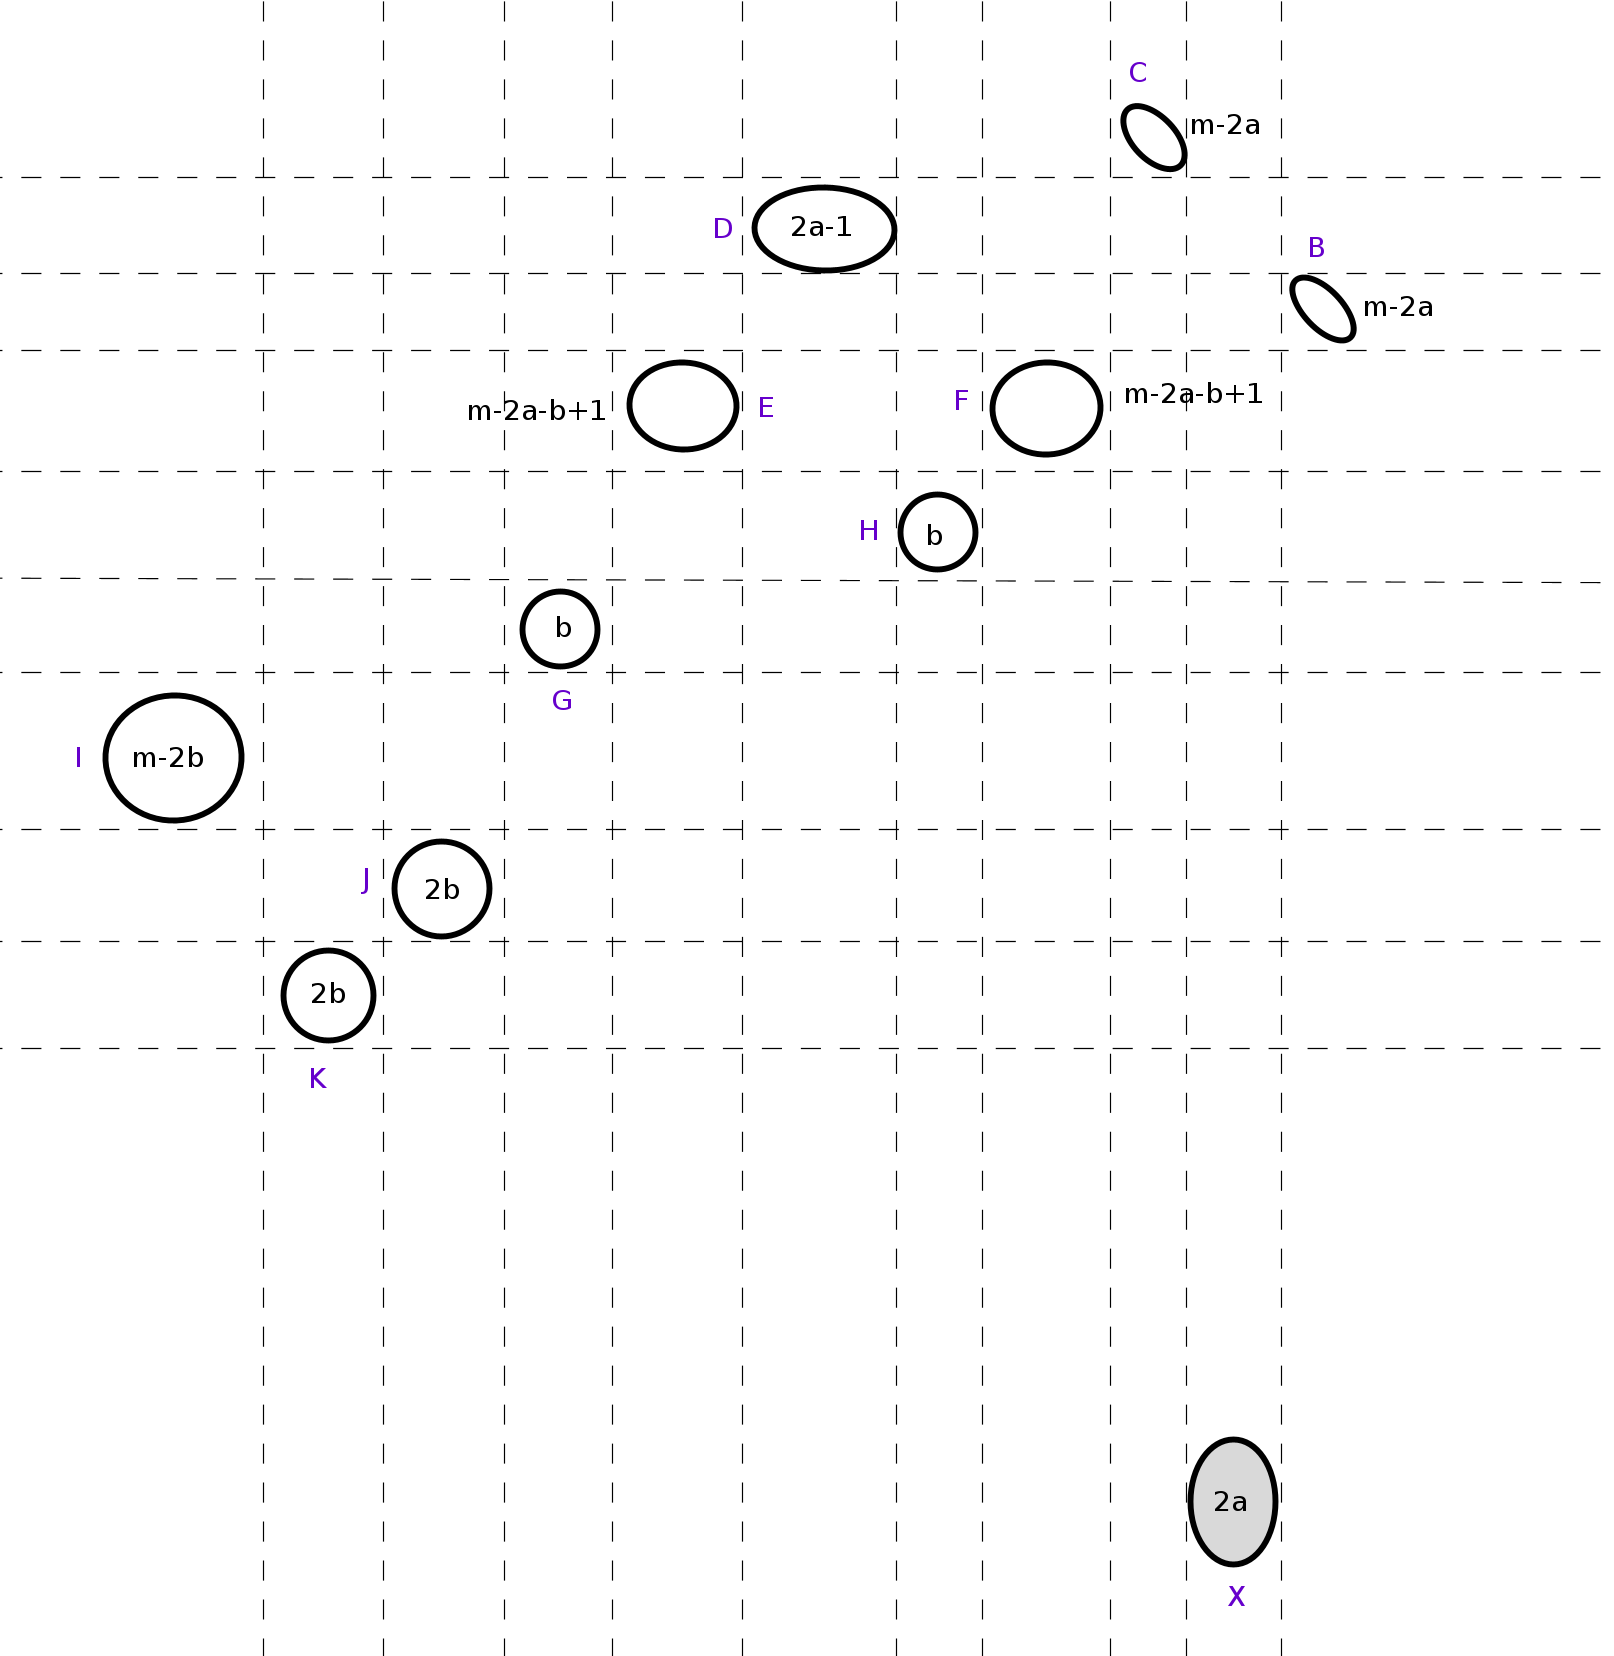
\includegraphics{abra3.png}
    \caption{The vertical strip of a $2a$-set $X$}
    \label{gigasok}
\end{figure}



Now let $S$ be a 2-shallow hitting set, and suppose indirectly that $X$ does not contain an element from $S$. Then $B$ contains a point from the hitting set, because $B\cup X$ is captured by a vertical strip of size $m$. Take the largest $k$ such that $b_{k}\in S$, and take $B'=\{b_{k+1},\ldots,b_{m-2a}\}$, and $C'=\{c_1,c_2,\ldots,c_k\}$. Then $B'\cup C'\cup X$ is captured by a vertical strip, $|B'\cup C'\cup X|=m$, and $S\cap(B'\cup X)=\emptyset,$ so $S\cap C'\ne \emptyset$. Therefore, $|S\cap(\{b_k\}\cup B'\cup C')|\ge 2,$ which implies that $D\cap S=\emptyset$, because $\{b_k\}\cup B'\cup C'\cup D$ is captured by a horizontal strip.

Observe that $|D\cup E\cup G|=|D\cup E\cup H|=|D\cup F\cup H|=m$, and that these sets are all captured by an axis-parallel strip, thus $E \cup G$, $E \cup H$ and $F \cup H$ each contain a point from $S$. Notice that $a-\frac{b}{2}=m-2a-b+1=|E|=|F|$, so $|E\cup F\cup H|=2a$, which implies $\big|(E\cup F\cup H)\cap S\big|\le 1$, because otherwise $E \cup F \cup H \cup B$ would form a hyperedge of cardinality $m$ containing at least 3 points from the hitting set.

% This implies $E\cap S=\est$, hence $G$ and $H$ contain a point from S, and so $I\cap S=\est$. This means that $J$ and $K$ has a point from $S$, $L\cap S=\est$. So if $m\ge 6b$, then $I\cup L$ form a strip of size $2m-6b\ge m$ without a point from the hitting set, which is a contradiction.


 This implies $E\cap S=\emptyset$, hence $G$ and $H$ each contain a point from S, so $I\cap S=\est$. Thus $J$ and $K$ each contain a point from $S$, so $|S\cap(G\cup J\cup K)|\ge3.$ Assuming $m\ge 5b$, $G\cup J\cup K$ can be extended to a hyperedge of cardinality $m$, which is a contradiction.
\end{proof}

\end{document}
